\chapter{Using the ENRAM software}

Make sure you have your virtual machine running (as in Figure~\ref{fig:screenshot-19}). 

Start the File Manager by clicking on the desktop icon labeled `File Manager'. In the file manager window, double-click on the directory called `enram' to inspect its contents.

Start a terminal by double-clicking the desktop icon labeled `Terminal'. This should bring up a terminal program (Figure~\ref{fig:screenshot-24}). In the terminal window, use the \texttt{cd} command to change directory into the `enram' directory. 

\begin{figure}[ht]
  \centering
    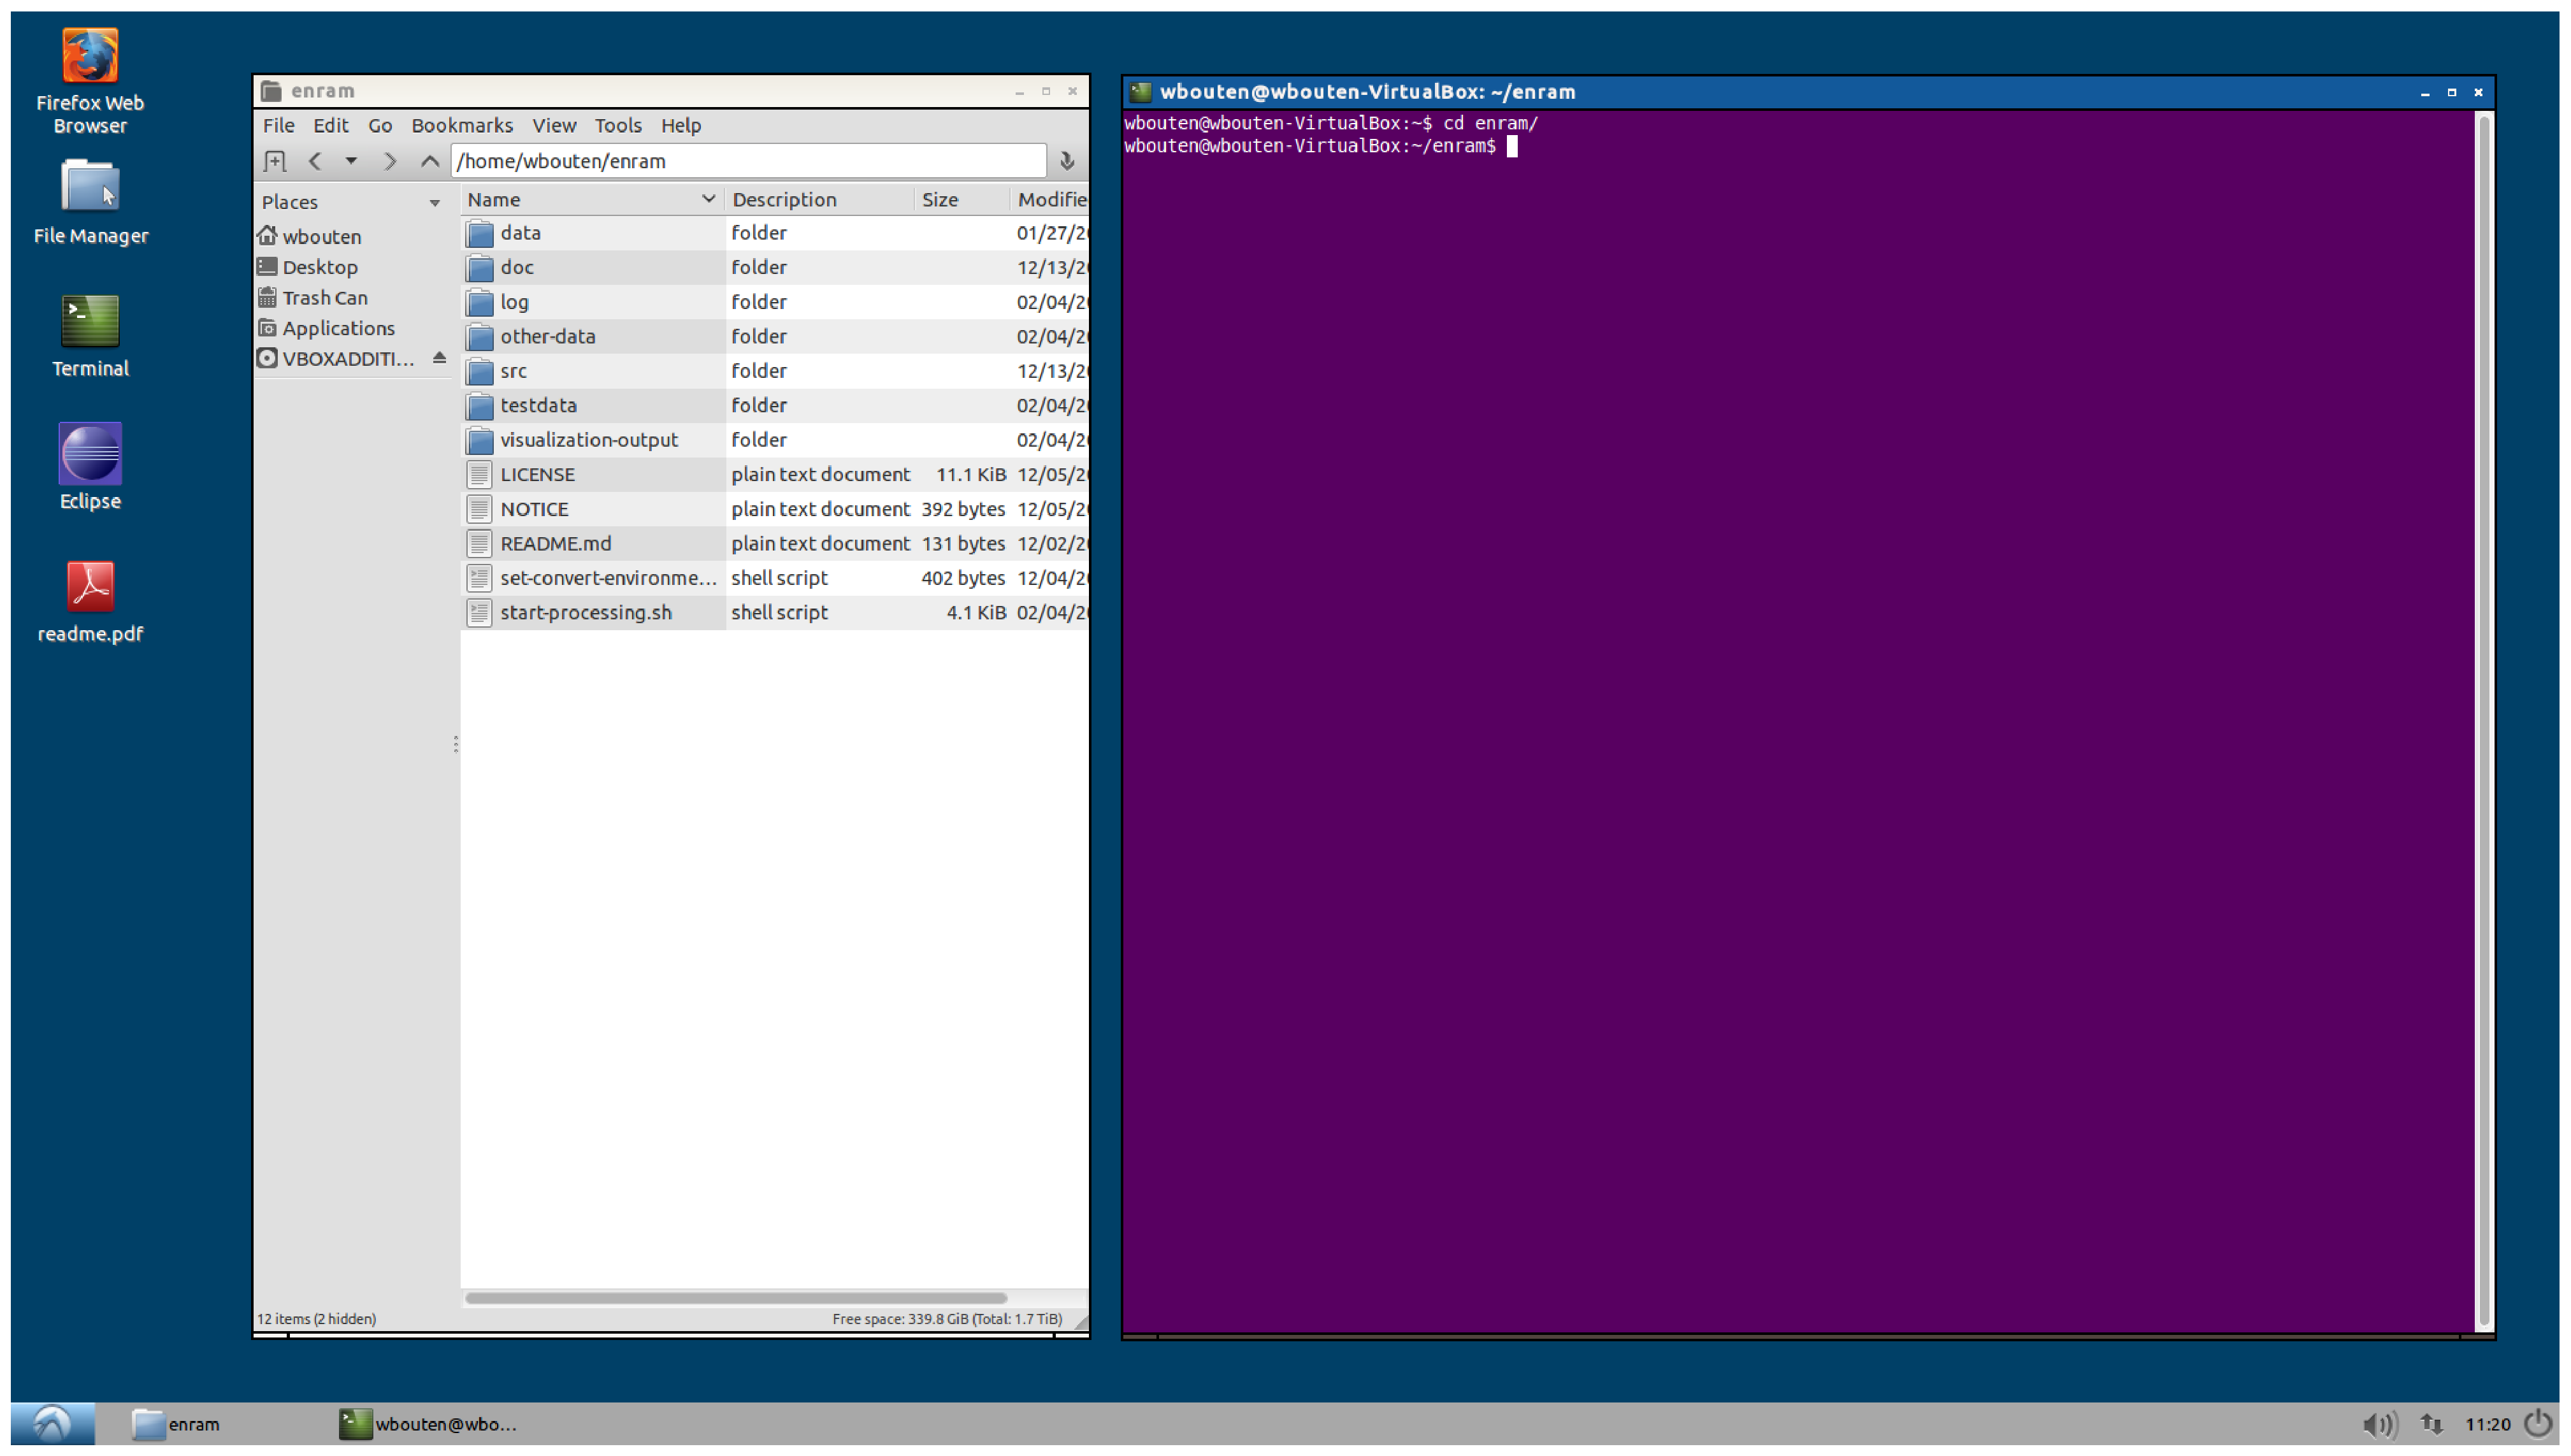
\includegraphics[width=0.85\linewidth , keepaspectratio]{./../eps/screenshot-24.eps}
  \caption{}
  \label{fig:screenshot-24}
\end{figure}


You can now start the ENRAM workflow as follows. Type:\\
\texttt{. ./start-processing.sh}

(But make sure to type it exactly as it is displayed here, including the leading dot).

The terminal will then first ask you whether you want an interactive session or you want to start processing in batch mode; then it will ask you to select either the test data set or the full data set (Figure~\ref{fig:screenshot-25}).

\begin{figure}[ht]
  \centering
    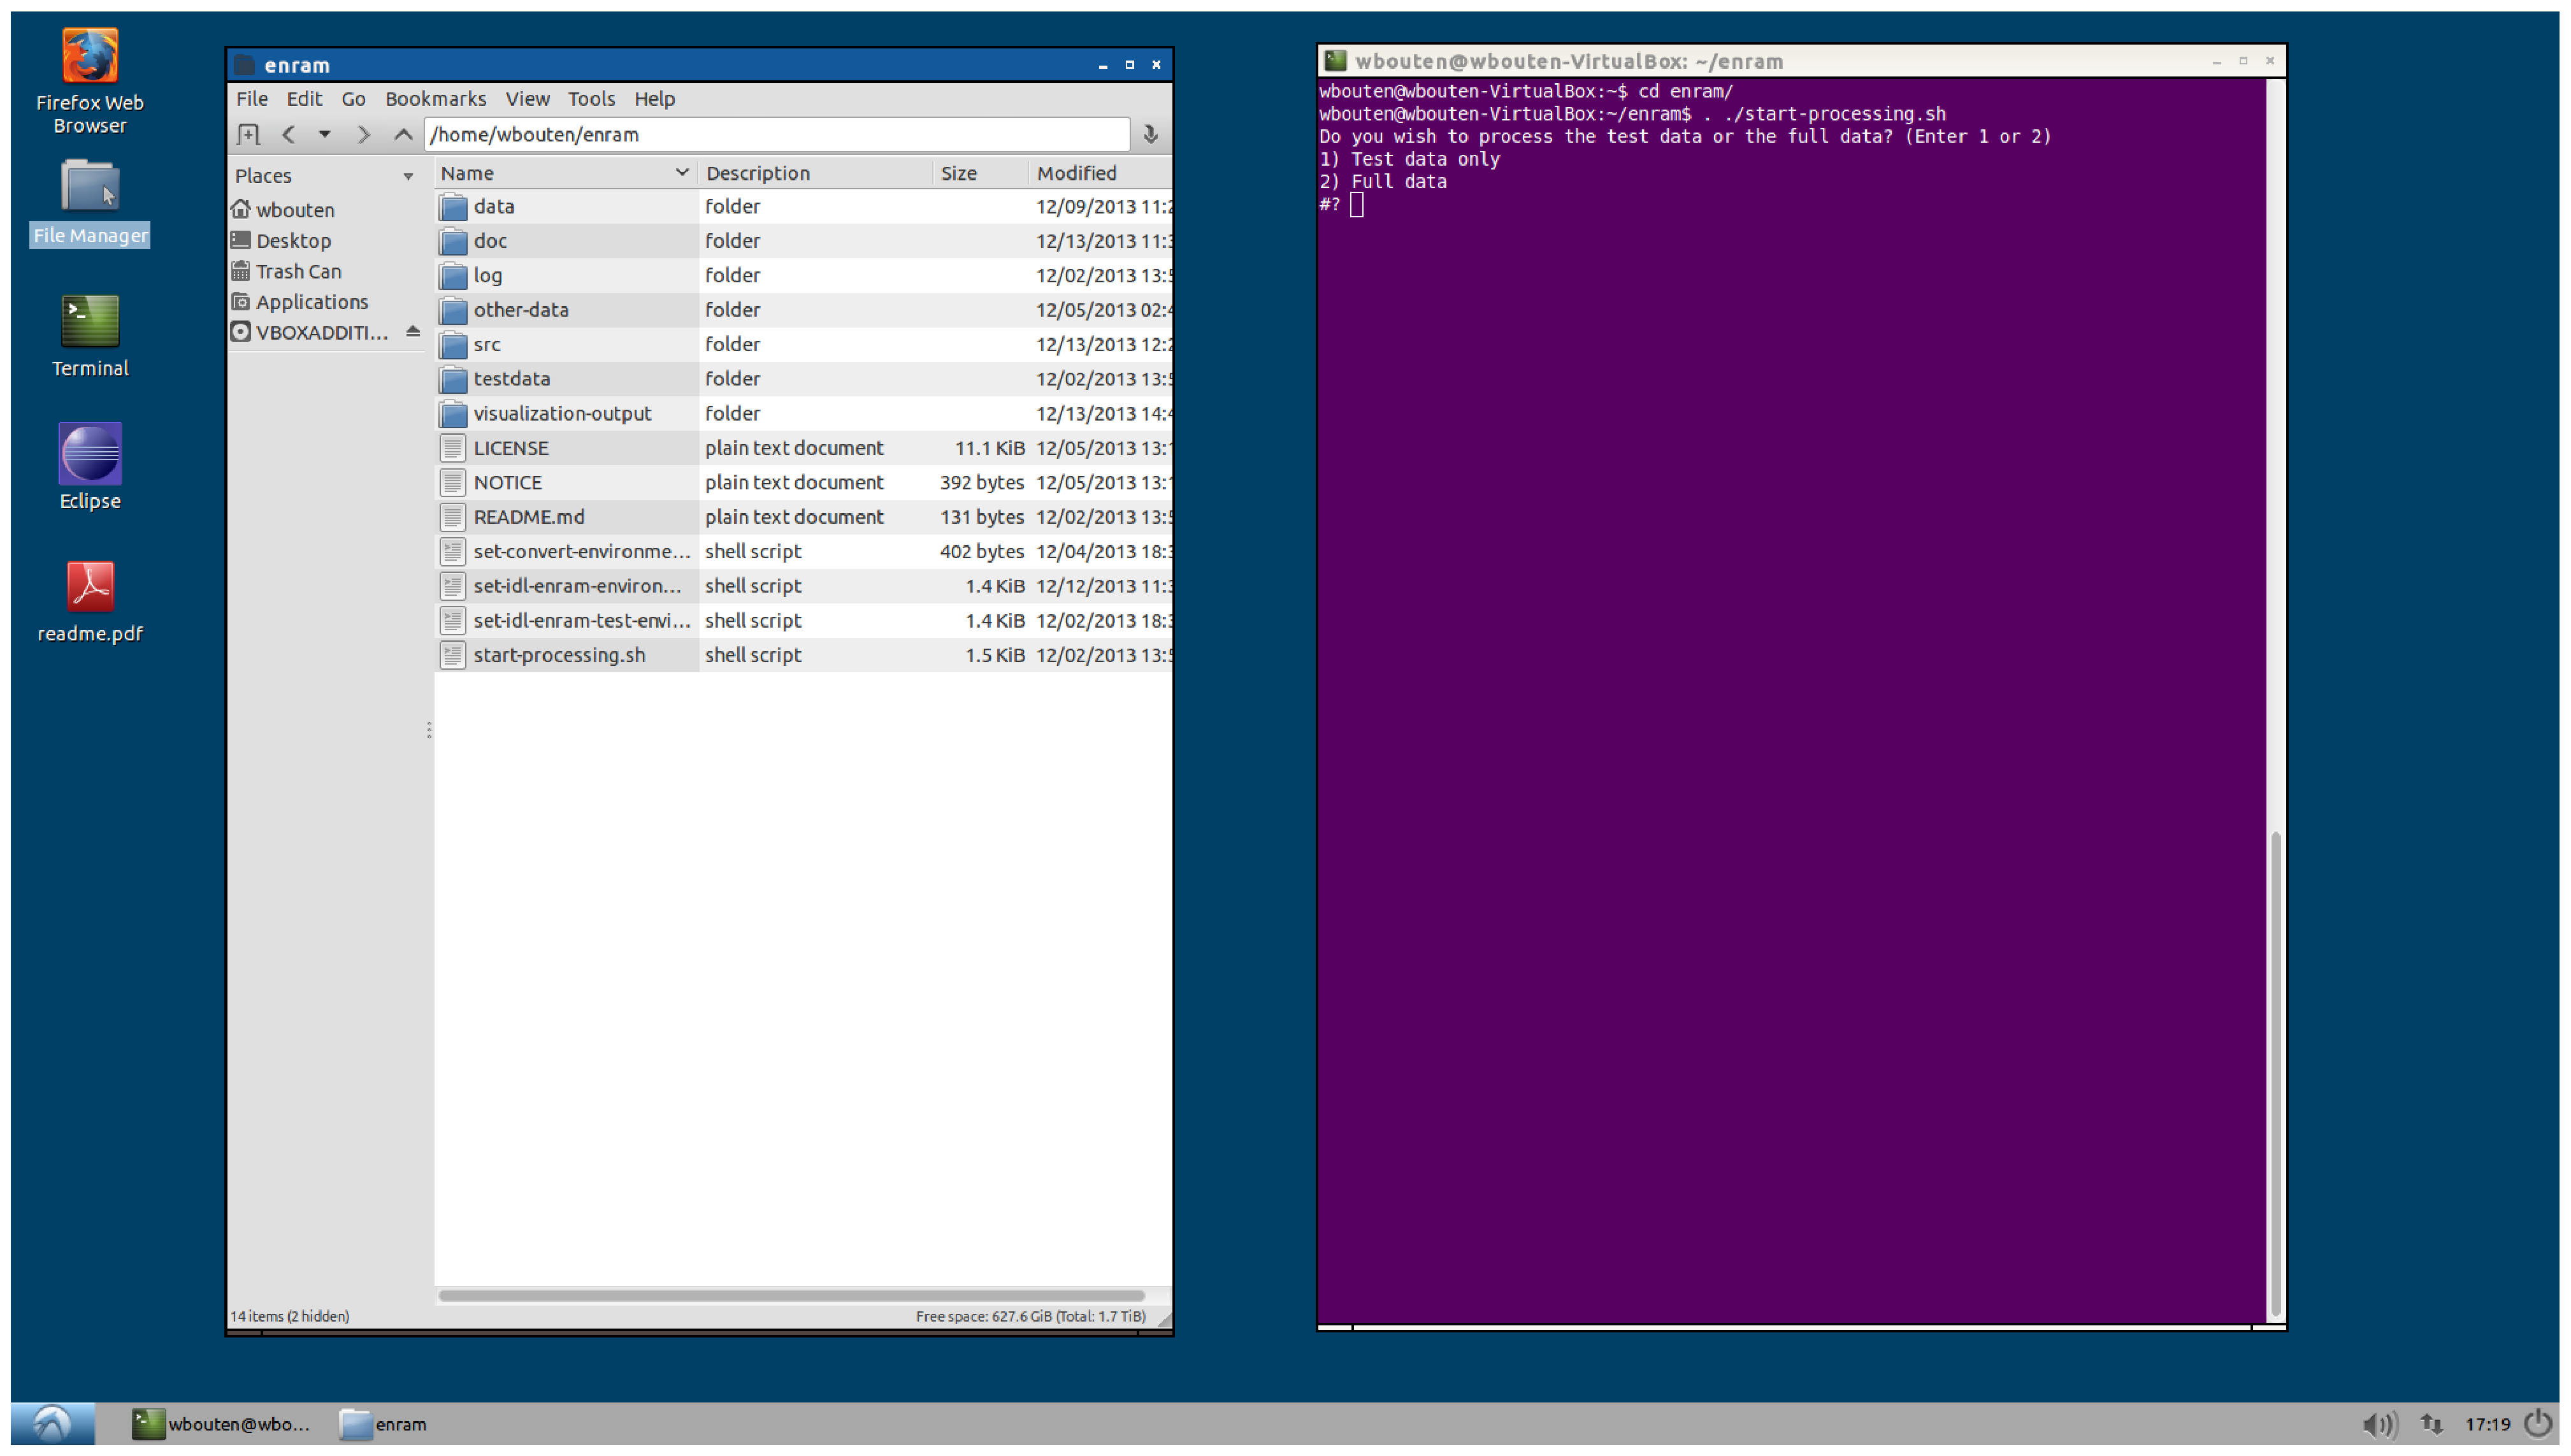
\includegraphics[width=0.85\linewidth , keepaspectratio]{./../eps/screenshot-25.eps}
  \caption{}
  \label{fig:screenshot-25}
\end{figure}

Answer `1' or `2' and press Enter at each question. The terminal will now set up the necessary environment variables.

If you chose to process the data in batch mode, you can use the Firefox web browser to view the batch program's feedback (Figure~\ref{fig:screenshot-26}) while the terminal program is running. Just navigate to `file:///home/wbouten/enram/log/stderr.txt' and `file:///home/wbouten/enram/log/stdout.txt'. Note that these locations have been added to the bookmarks, so if you just type `stderr' or `stdout' in Firefox's URL bar, it should suggest the corresponding files automatically.

\begin{figure}[ht]
  \centering
    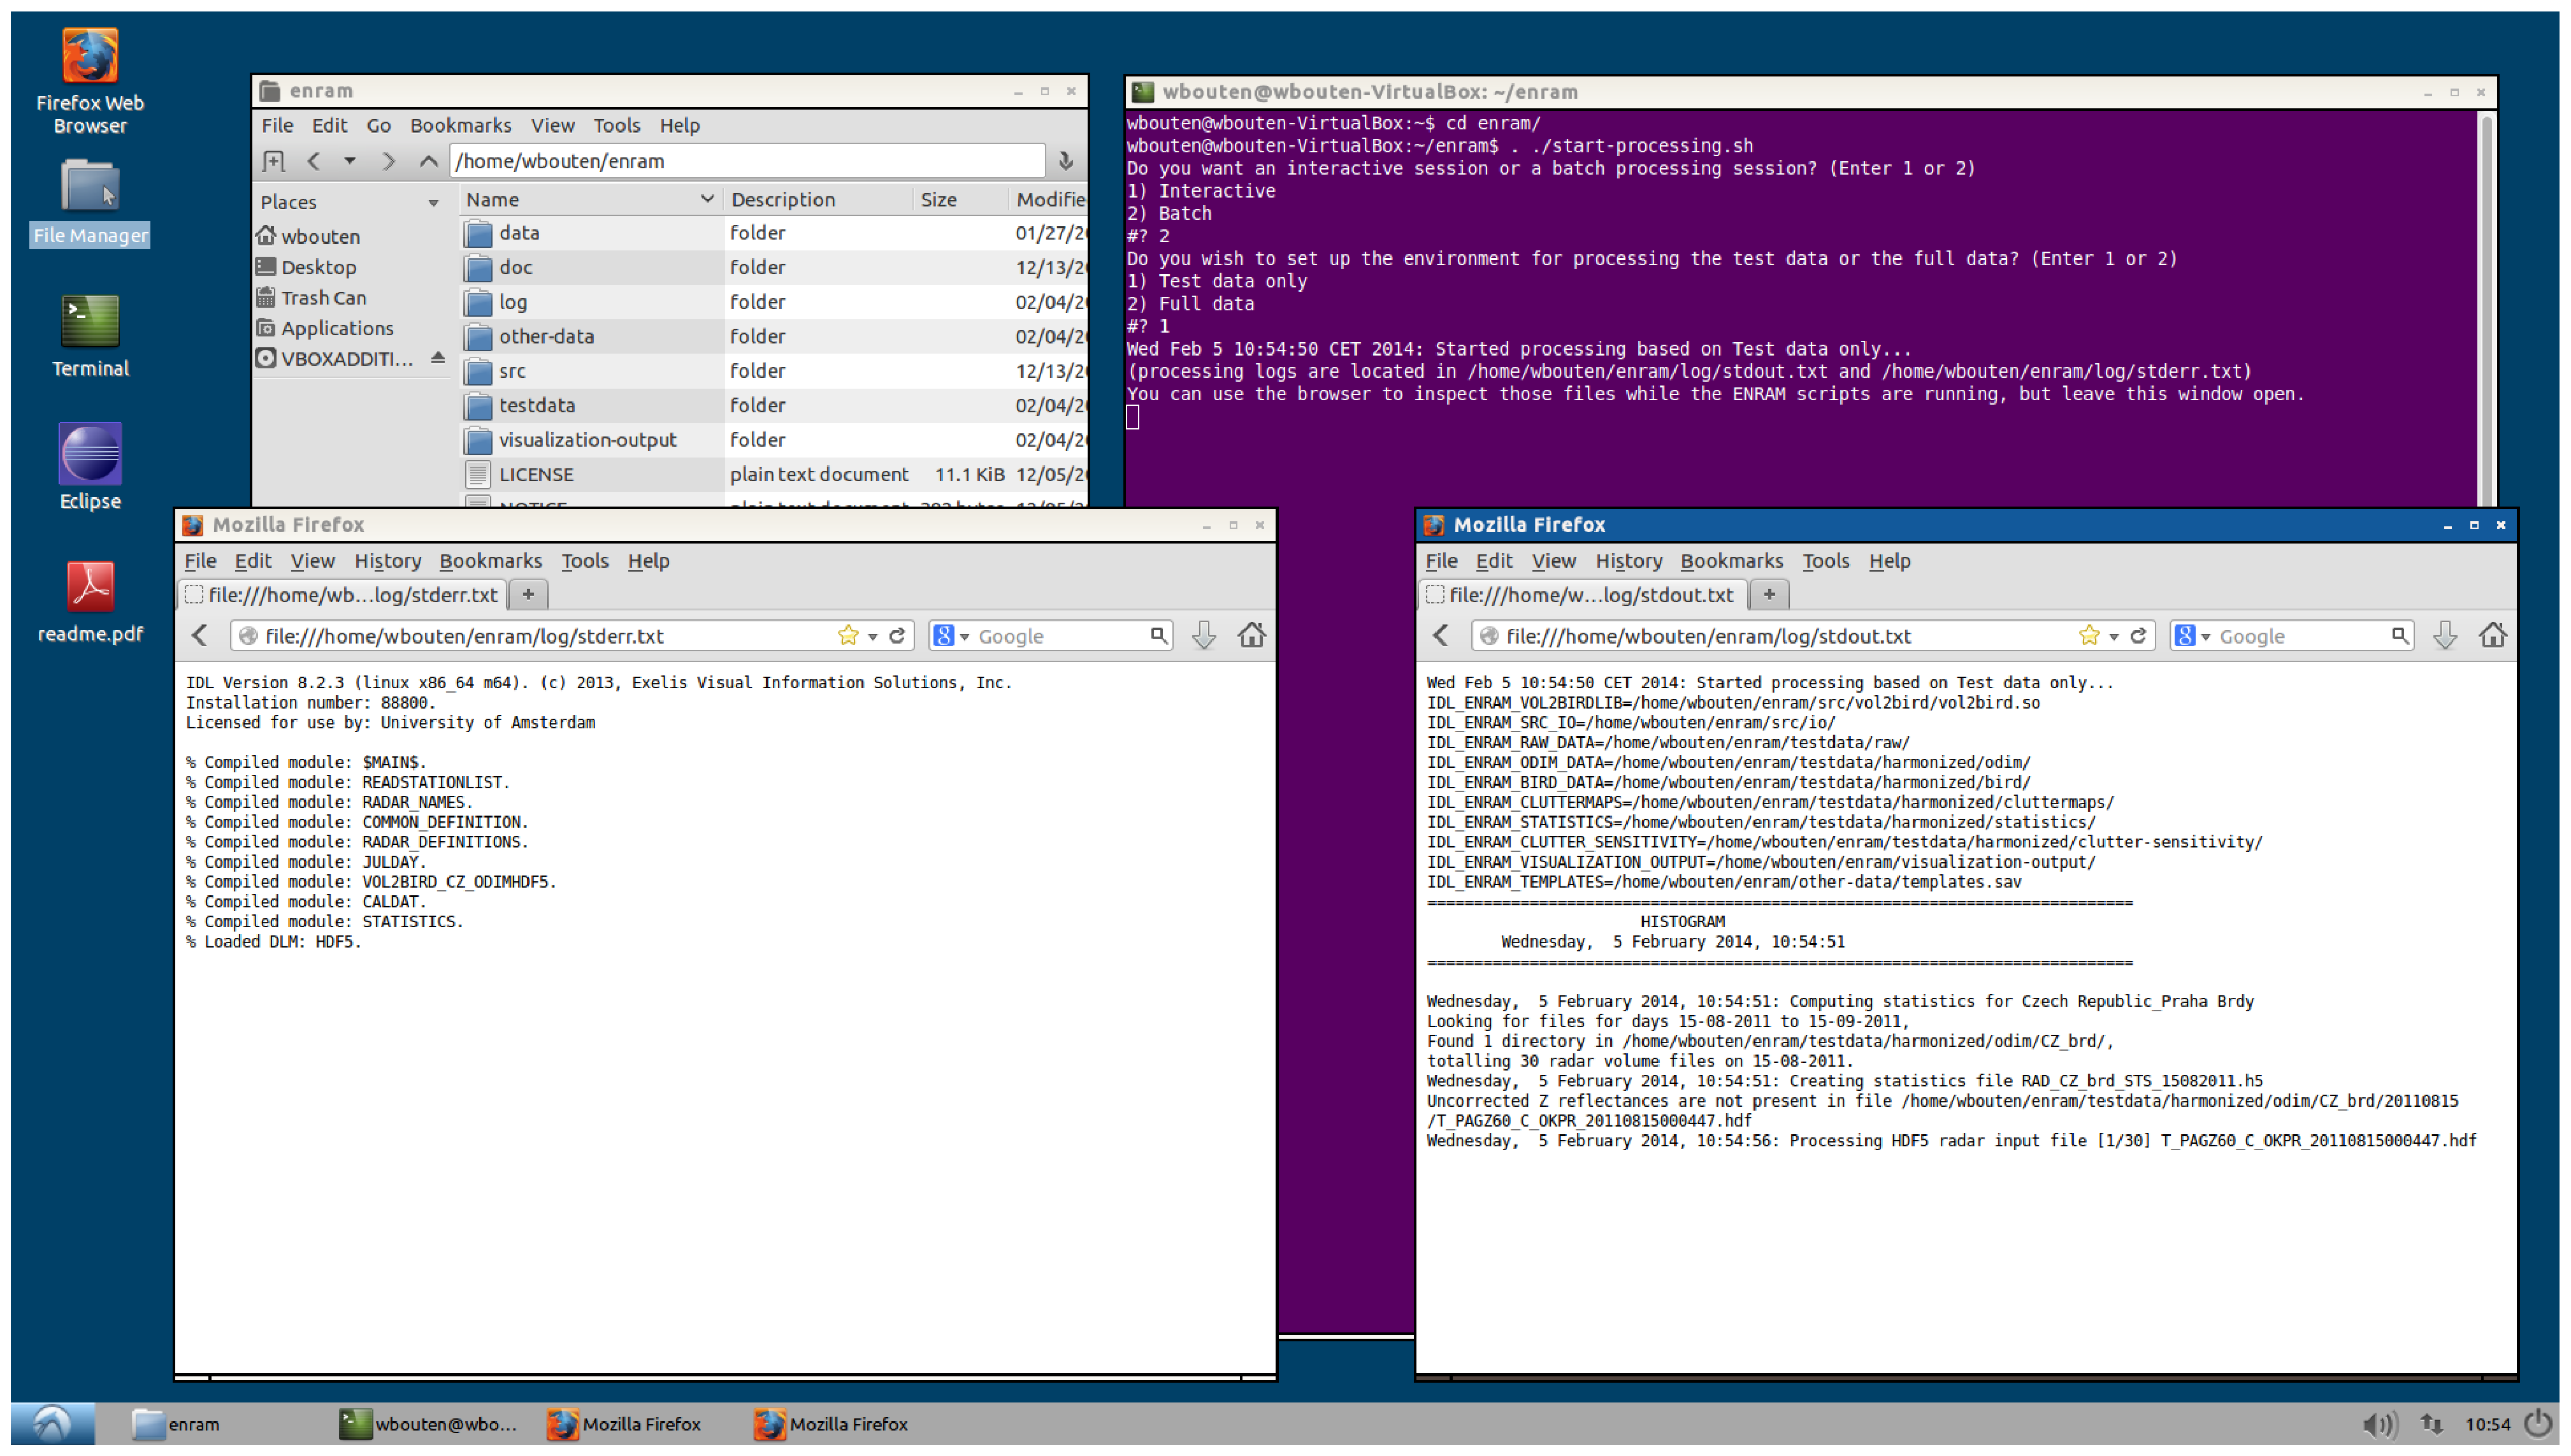
\includegraphics[width=0.85\linewidth , keepaspectratio]{./../eps/screenshot-26.eps}
  \caption{}
  \label{fig:screenshot-26}
\end{figure}
